\chapter{Lab work} 
\pagenumbering{arabic}
\label{chap_Intro}
This section introduces the lab work and implementation of the logger. The focus is on the time module as this is the primary focus for analysis during this experiment.

In this lab we created a logging system which can be used to log events in a distributed system without printing messages in the wrong order. As nodes usually experience different latencies in such a system it can happen that the log for sending a messages arrives after the log for the retrieval of the same message. We must in that case make sure that they are printed in reverse order to give a reasonable representation of system states.

Multiple workers that run in parallel on one machine represent the separate nodes in this lab. In the example they do not actually perform any real activity, but only simulated delays affect them. They will periodically send messages to each other and also log send and receive events to the logger process. As we have introduced artificial delays in the system we have a much higher probability of events happening in reverse order as they arrive to the logger process.

When a message arrives to the logger module it checks if it is safe to print using Lamport time or by using vector clocks. The logics for the clocks is completely contained in the time module but worker nodes must make use of this interface. The inner workings here are introduced in greater details under section \ref{time-module}. If messages still are unsafe when they arrive to the logger module they are saved in a priority queue for later printing. This queue is rechecked each time a new message is received which may update the overall time state and allow for more messages to be printed. This means that we can print messages during execution and still make sure they are at least casually ordered.

 
\section{The Time Module}
\label{time-module}
The time module contains code for representing both timestamps and a global clock (kept by the logger process). Each node will keep track of the Lamport time itself and each time a log message is received, we can add this information to the global clock. Each time a event happens in a system using Lamport time our time stamp will update. If the event involves sending a message to another node, we will always include our own time stamp and the receiving node will select the highest of it's own and the received time stamp. It then increments this by one which means that the time is always increasing and a receive event will always have a larger number than the corresponding send event.

This module provides a interface to both increment, merge into the largest time stamp and compare different time stamps to find the lesser of them. In addition to the time management for the nodes it also provides the interface for the logger module that can update the global time with a new time and check if a message with a provided time stamp is safe to print. In the first version of the code (using regular Lamport time) this means that the time stamp must be lower or equal to the max seen for each process in the system. Time is in this case represented by a regular integer which can easily be compared and increased.
\[ T_{message} \leq T_{max}(p), \qquad \forall p \in processes \]

For the second version using vector clocks we still need to compare a incoming timestamp to each time stamp in the global clock but the way we represent and compare time stamps is different. Here we consider a time stamp smaller if each index in the vector is smaller or equal to the other vector.
\[ T_{message}[i] \leq T_{max}[i], \qquad \forall i \in [0, \text{nr of workers} ] \]
where $ T[i] $ represents the vector index i in time stamp T.

\section{Problems}
One problem with this method is that many messages may be stored in the queue as they are still not considered safe. Take the following example:

\textit{
	We have 3 nodes (A, B and C) that are connected in a network. Process A and B frequently communicate with each other but C never sends or receives anything. Process C will have a very low time stamp (0) and all messages from A and B are considered unsafe until C starts to communicate. In reality it is not a problem to print messages from A and B as they are independent of C but the system can not detect this in the current state.
}

This is a bigger problem for the version using a single integer to represent the time stamp as we can't make a difference between the different nodes when we only have a single number to look at. In the vector version it is still possible to print messages from A and B in this case as we compare the clock state to the lowest for each node instead of the lowest of the entire system.

We can see this in action by looking at the queue size during execution. Figure \ref{fig:lamport-queue} illustrates this for the regular version where each node is only responsible for keeping a single lamport clock. To create the graphs the test program was ran with the parameters

\begin{lstlisting}
	test:run(50,1000).
\end{lstlisting}

\begin{figure}[h]
\centering
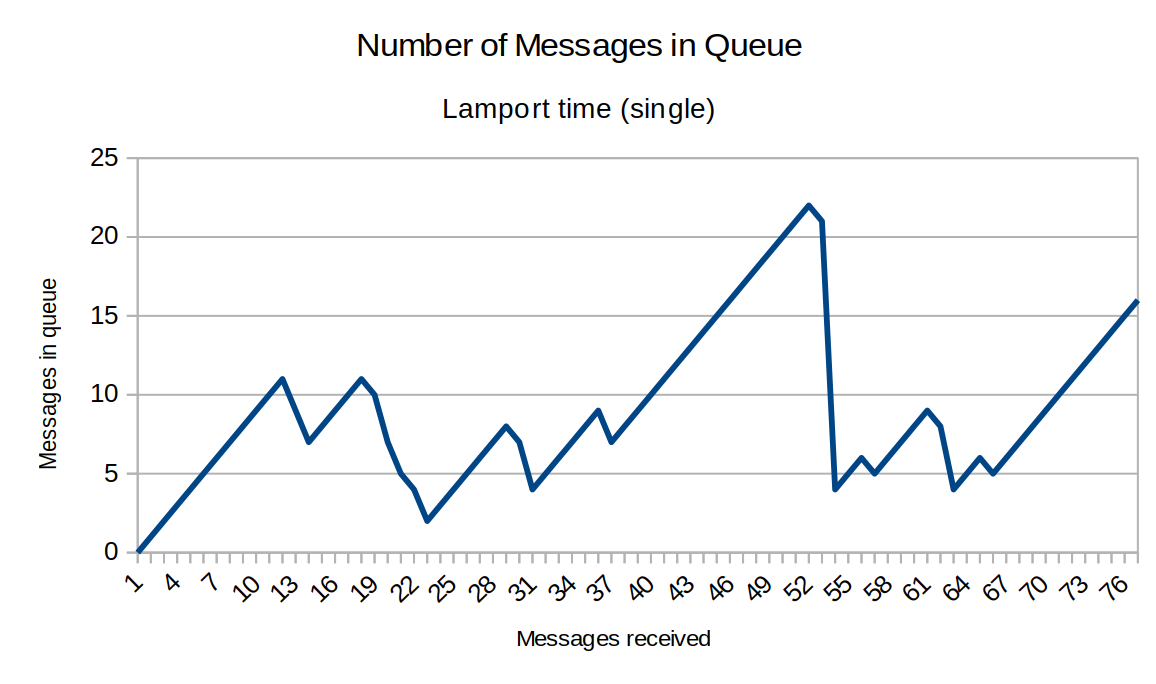
\includegraphics[width=0.8\linewidth]{res/lamport-queue}
\caption{Illustration of queue size for the version using only a single lamport clock per node}
\label{fig:lamport-queue}
\end{figure}

The second experiment was instead using the vector clocks which did not significantly improve performance. We can see that the benefits from using vector clocks can be quite small (if any at all) if all nodes in the system frequently sends messages to each other. The result from this experiment is shown in figure \ref{fig:vector-queue}.

\begin{figure}[h]
\centering
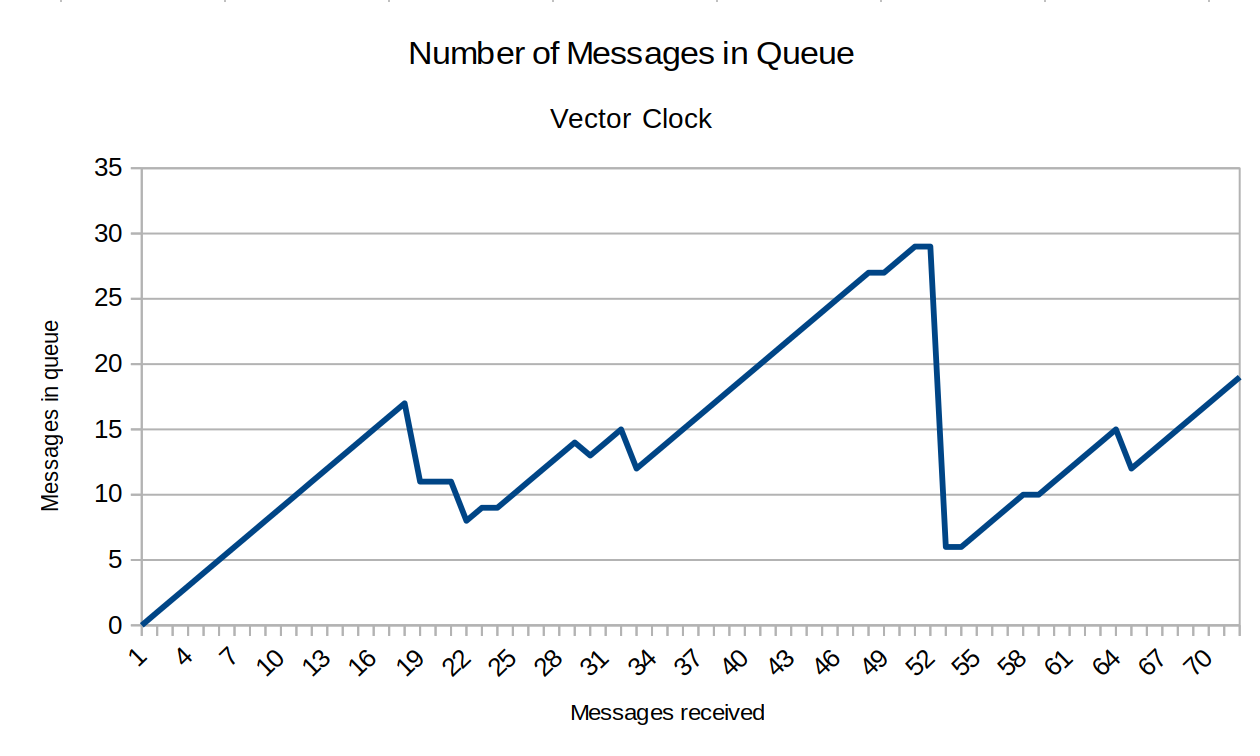
\includegraphics[width=0.8\linewidth]{res/vector-queue}
\caption{Illustration of queue size for the vecotr clock}
\label{fig:vector-queue}
\end{figure}

In a worst case scenario we can have all messages waiting for one of the earlier messages which means that no messages can be printed. This holds true for both the version using a single Lamport clock and the vector clock, however the risk is much greater for the single clock version as all processes must send an equal number of messages here or always communicate with all other nodes. In the experiments we conducted here, values were a bit extreme with up to one second of delay before sending the log message. Each experiment only lasted for five seconds in total which means that many messages could potentially build up in the log. Even with the extreme configuration we can see that the number of messages will remain quite stable and never reaches far above 30. This is illustrated in figure \ref{fig:vector-queue-over-time} which shows the queue size during a execution which lasted 30 seconds.

\begin{figure}[h]
\centering
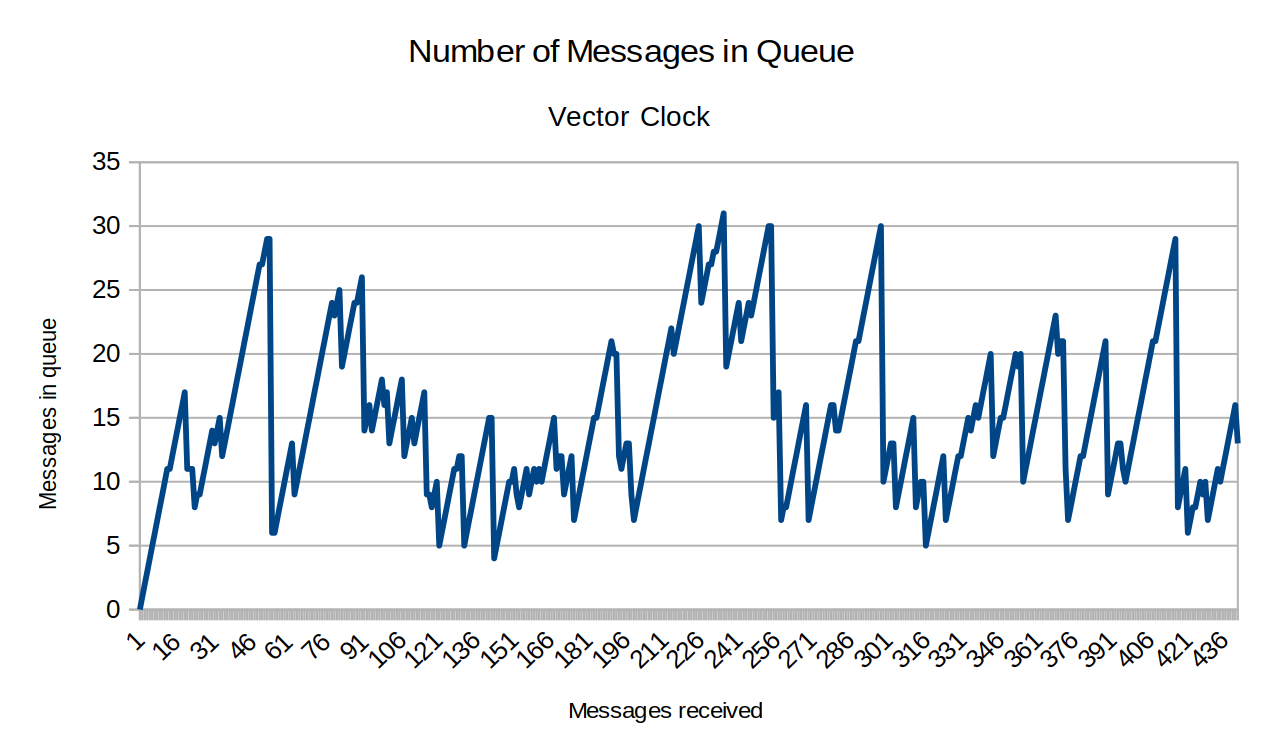
\includegraphics[width=0.8\linewidth]{res/vector-queue-over-time}
\caption{Illustration of queue size over time for the vector clock}
\label{fig:vector-queue-over-time}
\end{figure}

Another possible problem with using Lamport time is that the order is not absolute. We know for sure that if one event happened-before another it will have a lower number. Happened-before is defined as a message beeing sent from the first process to the second.
\[ E_1 \rightarrow E_2 \Rightarrow V(E_1) \leq V(E_2) \]
This means that we only order logs that are directly correlated with event. The actual time is not considered here with means that they might be printed out of order compared to when they actually happened. On the other hand the global state will always be consistent which is important when you try to assess the application for debugging purposes.





